%{
% \documentclass[12pt, ngerman]{/Users/dominik-cau/Documents/Lernen/Uni/Promotion/Lehre/Latex-Vorlage/ExamClass}
% \documentclass[12pt, english]{AssignmentClass}
\documentclass[12pt, ngerman]{AssignmentClass}

%----------------------------------------------------------------------------------------
%	PACKAGES AND OTHER DOCUMENT CONFIGURATIONS
%----------------------------------------------------------------------------------------

% Template-specific packages
\usepackage[utf8]{inputenc} % Required for inputting international characters
\usepackage[T1]{fontenc} % Output font encoding for international characters
\usepackage{mathpazo} % Use the Palatino font
\usepackage{graphicx} % Required for including images
\usepackage{amsmath}
\usepackage{booktabs} % Required for better horizontal rules in tables
\usepackage[normalem]{ulem}
\usepackage{listings} % Required for insertion of code
\usepackage{siunitx}
\usepackage{array}
\usepackage{pnets}
\newcolumntype{Y}{>{\centering\arraybackslash}X}
\newcolumntype{C}[1]{>{\centering\arraybackslash}p{#1}}
\usepackage{comment}
\DeclareMathAlphabet{\mathpzc}{OT1}{pzc}{m}{it}
\useunder{\uline}{\ul}{}

% Underline %
\usepackage{contour}
\usepackage{ulem}

% new column types
\usepackage{array}
\newcolumntype{L}[1]{>{\raggedright\let\newline\\\arraybackslash\hspace{0pt}}m{#1}}
\newcolumntype{C}[1]{>{\centering\let\newline\\\arraybackslash\hspace{0pt}}m{#1}}
\newcolumntype{R}[1]{>{\raggedleft\let\newline\\\arraybackslash\hspace{0pt}}m{#1}}
\usepackage{graphicx,multirow}
\usepackage{wrapfig}
\setlength\intextsep{0pt}
\usepackage{stackengine}
\newcommand\xrowht[2][0]{\addstackgap[.5\dimexpr#2\relax]{\vphantom{#1}}}

% table
\usepackage{multirow}
\usepackage{tabularx}

% no indent
\setlength\parindent{0pt}

\renewcommand{\ULdepth}{1.8pt}
\contourlength{0.8pt}

\newcommand{\fancyuline}[1]{%
	\uline{\phantom{#1}}%
	\llap{\contour{white}{#1}}%
}

%----------------------------------------------------------------------------------------
%	ASSIGNMENT INFORMATION
%----------------------------------------------------------------------------------------
	
% \title{Hauptklausur} % Assignment title
\title{Matrikelnummer:} % Assignment title
\class{Generative KI} % Course or class name
\term{Sommersemester 2024 -- Hauptklausur} % Footer Line

% Exam Version
\includecomment{answerbox}
\excludecomment{solution}
% Solution Version
% \excludecomment{answerbox}
% \includecomment{solution}
%}

\begin{document}

\section*{Aufgabe 1 (Generative KI) \hfill 15 Punkte}

    % Aufgabenteil a
    \begin{enumerate}[a)]
		\item 
			\begin{minipage}[t]{\linewidth}
				\vspace{-0.61em}
				\begin{wrapfigure}[2]{r}{0.18\linewidth} 
					\raggedleft
					\texttt{(2 Punkte)}
				\end{wrapfigure}
                Generative KI-Systeme können verschiedene Arten von Daten gleichzeitig verarbeiten und können damit eine Vielzahl von Aufgaben lösen. Ergänzen Sie die folgende Abbildung um die Art von Daten, die ein Generatives KI-System verarbeiten kann. Tragen Sie die Art von Daten in die weißen Boxen ein.
			\end{minipage}
	\end{enumerate}
    
    \begin{figure}[h]
        \centering
        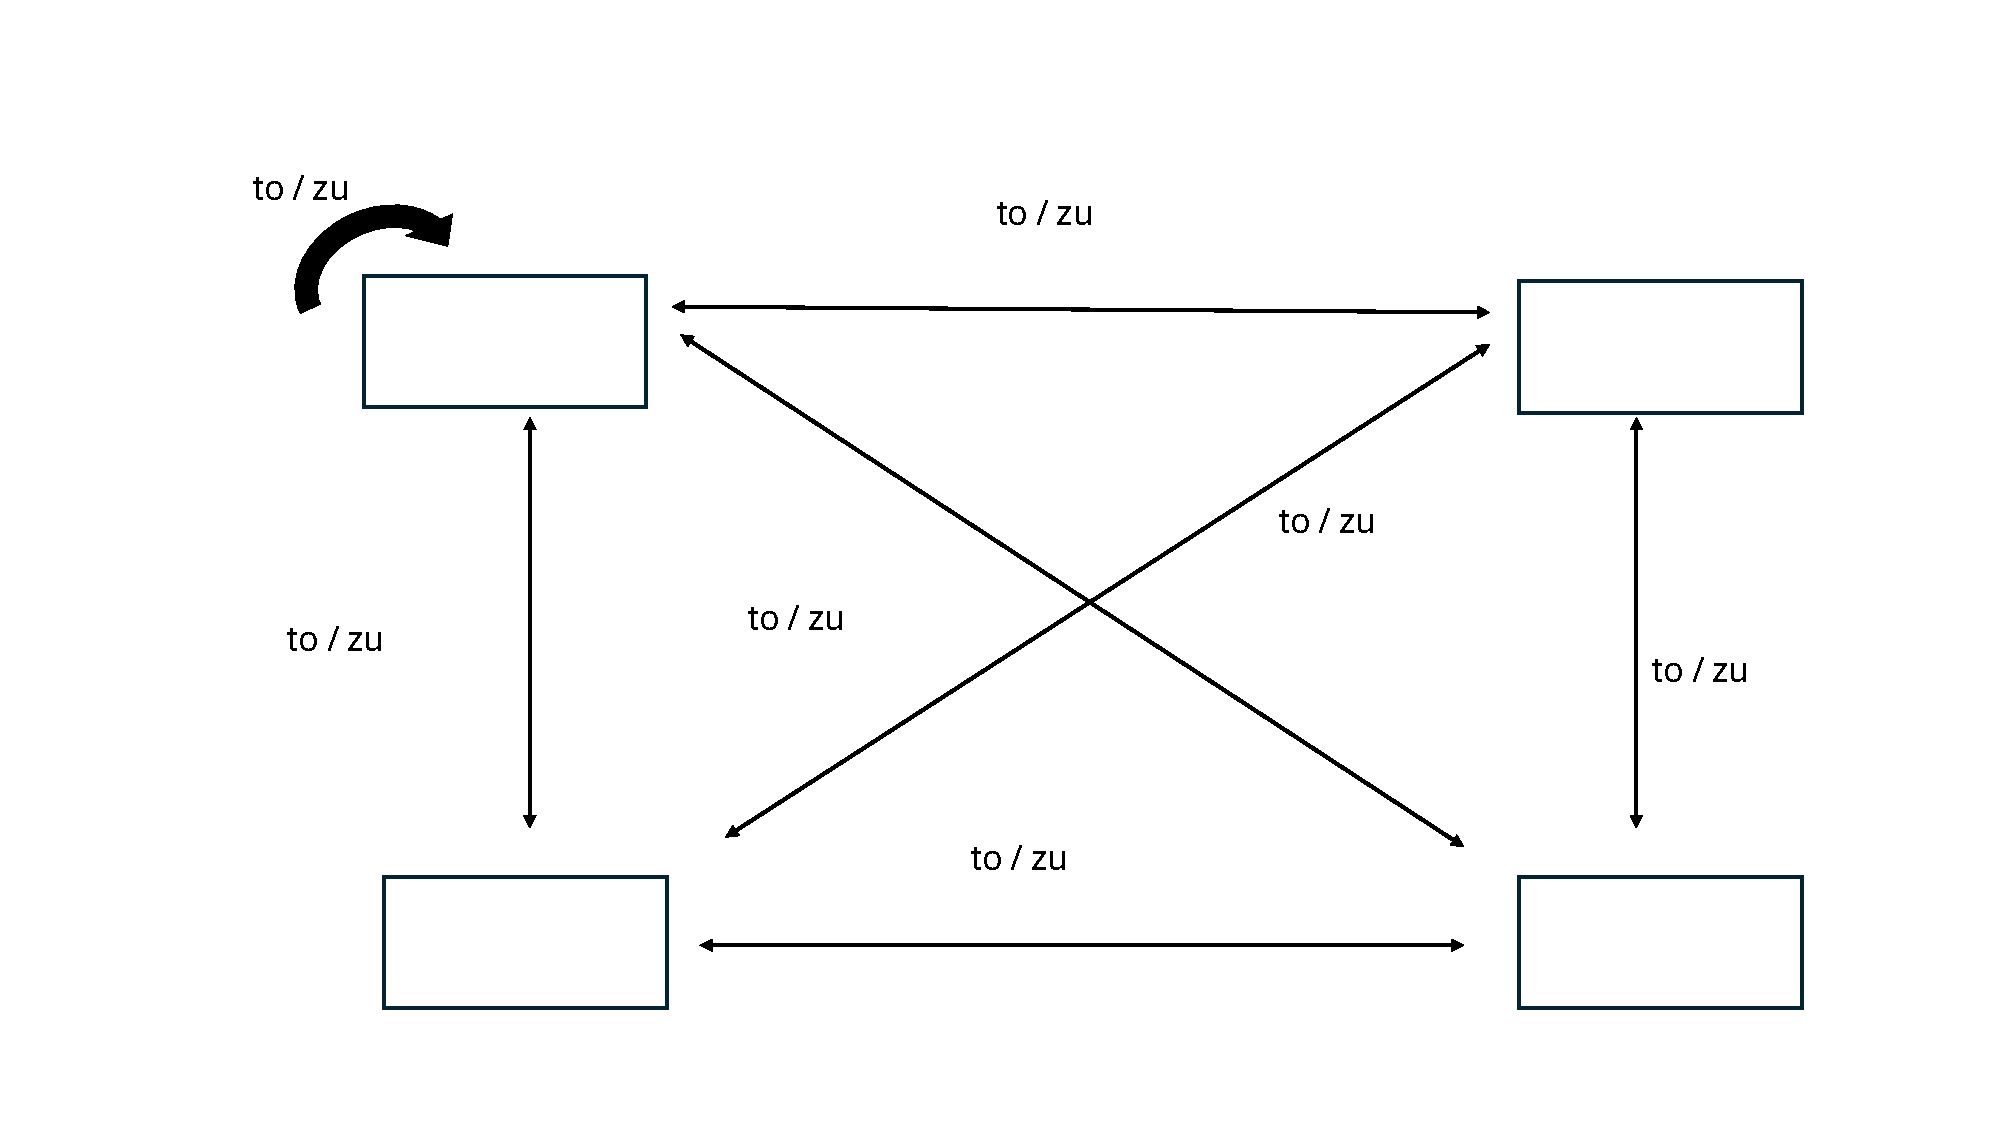
\includegraphics[width=1\linewidth]{media/Aufgabe 1/Aufgabe1.pdf}
        \label{fig:Aufgabe1}
    \end{figure}

	\begin{solution}
        \begin{figure}[h]
            \centering
            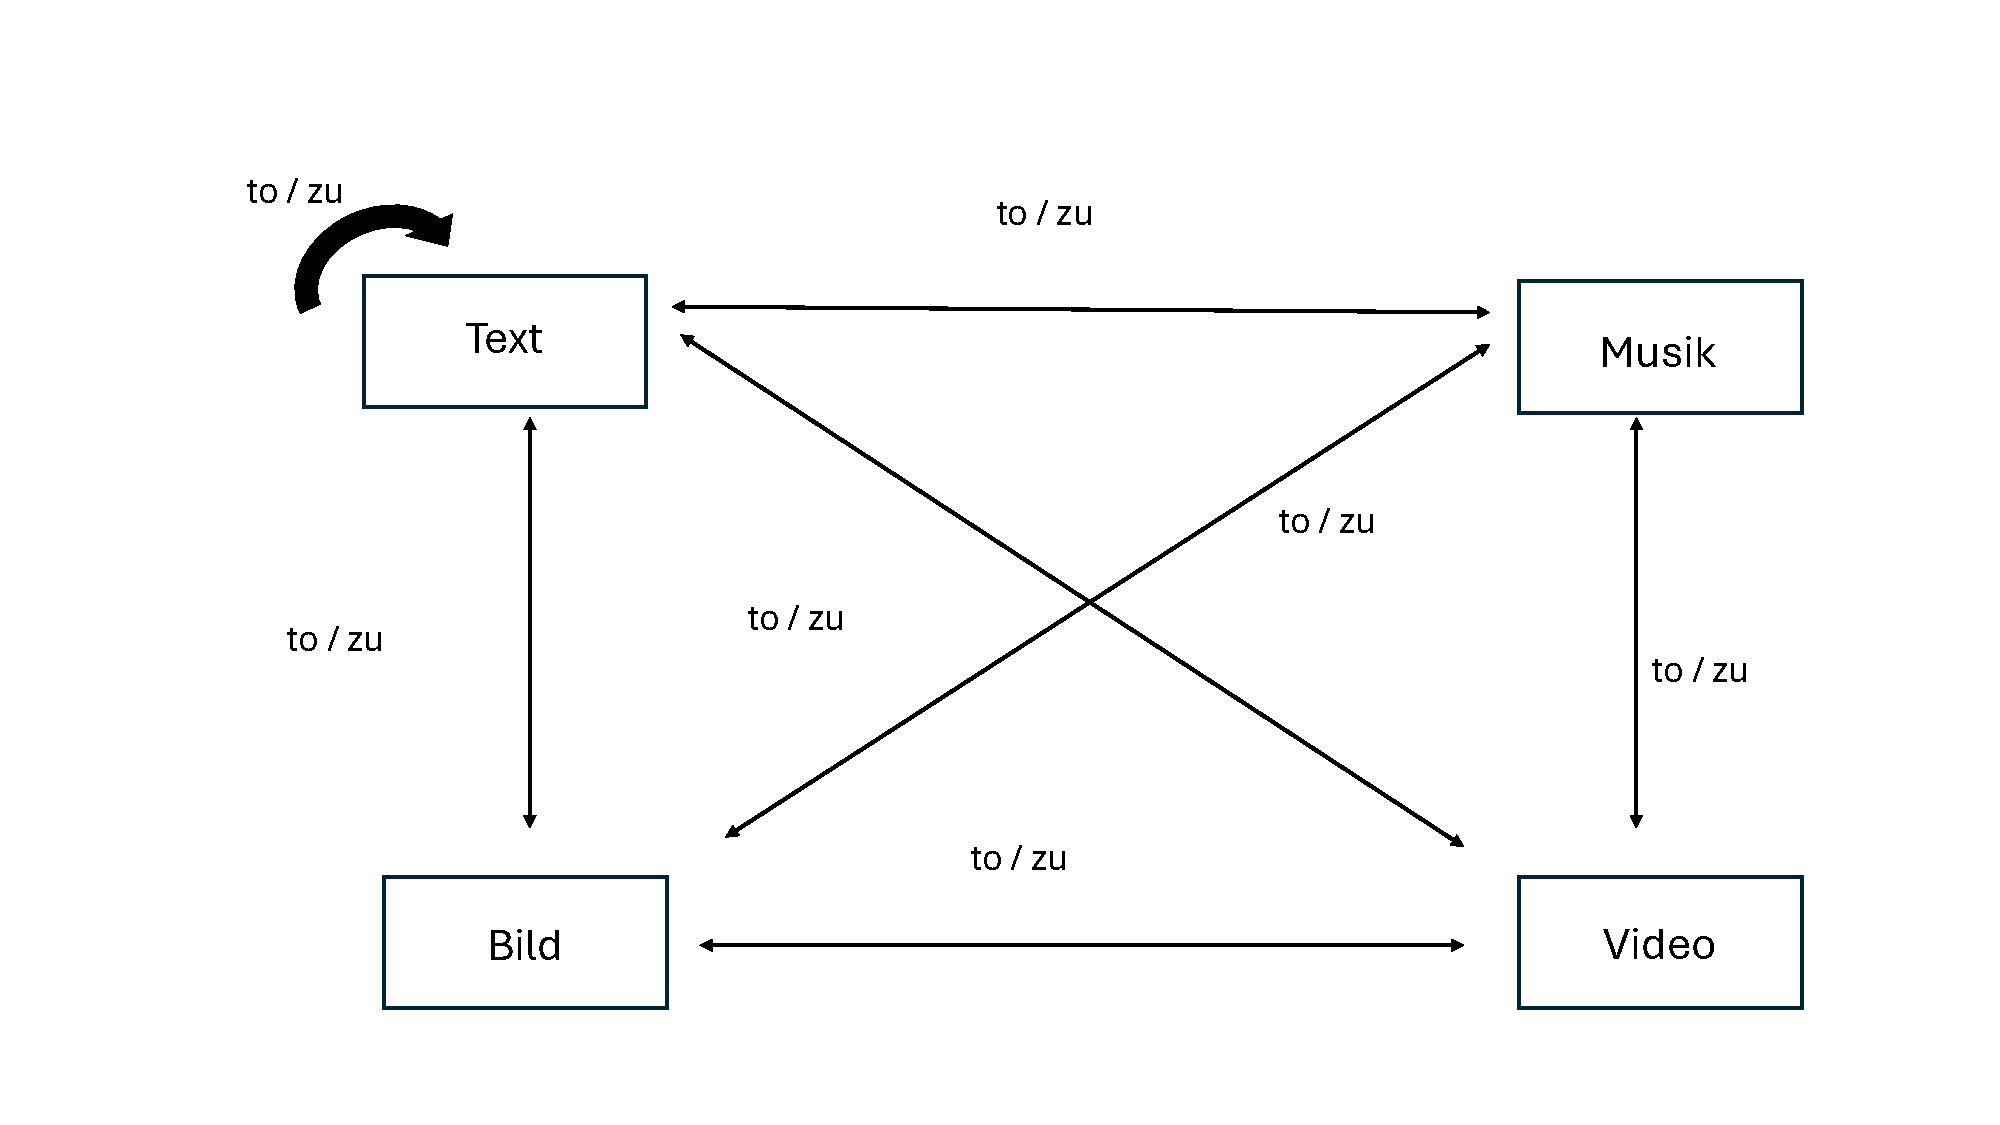
\includegraphics[width=\linewidth]{media/Aufgabe 1/Aufgabe1-Loesung.pdf}
            \label{fig:Aufgabe1-Loesung}
        \end{figure}
	\end{solution}

    % Aufgabenteil b
    \begin{enumerate}[b)]
		\item 
			\begin{minipage}[t]{\linewidth}
				\vspace{-0.61em}
				\begin{wrapfigure}[2]{r}{0.18\linewidth} 
					\raggedleft
					\texttt{(3 Punkte)}
				\end{wrapfigure}
                Nennen Sie drei Beispiele, was ein Sprachmodell von ChatGPT kann.
			\end{minipage}
	\end{enumerate}
 
	\begin{solution}
		\noindent
		\fbox{\parbox[c]{\textwidth}{
				\small
				\begin{tabular}{cp{13cm}}
                    & \textbf{Beispiele für Lösungen (Pro Beispiel 1 Punkt; max. 3 Punkte):}\\
					Punkte &\\
					1 & natürlich klingende Konversationen führen\\
					1 & Texte aller Art erstellen (Aufsätze, Gedichte, Zusammenfassungen, Kochrezepte etc.)\\
                    1 & Programmcode schreiben\\
                    1 & Texte übersetzen
				\end{tabular}
				\hspace{\textwidth}
		}}\\
	\end{solution}

    \begin{answerbox}
		\noindent
		\fbox{\parbox[c]{\textwidth}{
				\vspace{5cm}
				\hspace{\textwidth}
		}}\\
	\end{answerbox}

    \newpage

    % Aufgabenteil c
    \begin{enumerate}[c)]
		\item 
			\begin{minipage}[t]{\linewidth}
				\vspace{-0.61em}
				\begin{wrapfigure}[2]{r}{0.18\linewidth} 
					\raggedleft
					\texttt{(4 Punkte)}
				\end{wrapfigure}
                Generative KI-Modelle werden kontinuierlich verbessert und weiterentwickelt. Welche Besonderheiten unterscheiden grundsätzlich Generative KI-Systeme von „normalen“ KI-Systemen? Beschreiben Sie zwei besondere Eigenschaften.
			\end{minipage}
	\end{enumerate}
 
	\begin{solution}
		\noindent
		\fbox{\parbox[c]{\textwidth}{
				\small
				\begin{tabular}{cp{13cm}}
					& \textbf{Beispiele für Lösungen:}\\
                    Punkte &\\
					1 & Skalierbarkeit\\
					1 & Anpassbarkeit\\
                    1 & Prompt Engineering
				\end{tabular}
				\hspace{\textwidth}
		}}\\
	\end{solution}

    \begin{answerbox}
		\noindent
		\fbox{\parbox[c]{\textwidth}{
				\vspace{5cm}
				\hspace{\textwidth}
		}}\\
	\end{answerbox}

    % Aufgabenteil d
    \begin{enumerate}[d)]
		\item 
			\begin{minipage}[t]{\linewidth}
				\vspace{-0.61em}
				\begin{wrapfigure}[2]{r}{0.18\linewidth} 
					\raggedleft
					\texttt{(6 Punkte)}
				\end{wrapfigure}
                Vergleichen Sie zwei bestehende Sprachmodelle gegeneinander. Geben Sie für jedes Sprachmodell zwei signifikante Besonderheiten an. Dabei dürfen sich die Besonderheiten nicht widersprechen.                                                                                  
			\end{minipage}
	\end{enumerate}

    \begin{table}[h]
        \begin{tabularx}{\textwidth}{|p{0.25\textwidth}|l|X|}
        \hline
        Name des Modells  & Entwickler        & Besonderheiten    \\ \hline
        \multirow{6}{*}{} & \multirow{6}{*}{} & \multirow{6}{*}{} \\
                          &                   &                   \\
                          &                   &                   \\
                          &                   &                   \\
                          &                   &                   \\
                          &                   &                   \\ \hline
        \multirow{6}{*}{} & \multirow{6}{*}{} & \multirow{6}{*}{} \\
                          &                   &                   \\
                          &                   &                   \\
                          &                   &                   \\
                          &                   &                   \\
                          &                   &                   \\ \hline
        \end{tabularx}
    \end{table}

	\begin{solution}
		\noindent
        \begin{table}[h]
            \begin{tabularx}{\textwidth}{|p{0.25\textwidth}|l|X|}
            \hline
            Name des Modells  & Entwickler        & Besonderheiten    \\ \hline
            \multirow{3}{*}{} & \multirow{3}{*}{} & \multirow{3}{*}{} \\
            ChatGPT (Generative Pre-trained Transformer) & OpenAI & Im November 2021 als erstes Sprachmodell für die kostenlose Nutzung veröffentlicht. Basiert in der Pro-Version auf GPT-4, einem multimodalen Modell \\ \hline
            BERT (Bidirectional Encoder Representations from Transformers & Google & Bidirektionales Transformer-Modell. Kann Wörter durch ihren gesamten Kontext vorhersagen. Basis für eine Familie von KI-Modellen, die sich von GPT abgrenzt. Nützlich für viele Klassifikationsaufgaben. Wird z.B. in der Google-Suche eingesetzt.\\
            \hline
            \end{tabularx}
        \end{table}
	\end{solution}


\section*{Aufgabe 2 (Large Language Models) \hfill 10 Punkte}
    % Erklären Sie die Funktionsweise von Large Language Models.

    % Aufgabenteil a
    \begin{enumerate}[a)]
		\item 
			\begin{minipage}[t]{\linewidth}
				\vspace{-0.61em}
				\begin{wrapfigure}[2]{r}{0.18\linewidth} 
					\raggedleft
					\texttt{(2 Punkte)}
				\end{wrapfigure}
                Erklären Sie den Embedding Vektor. Wie ist er aufgebaut und welchen Zweck erfüllt er?
			\end{minipage}
	\end{enumerate}
 
	\begin{solution}
		\noindent
		\fbox{\parbox[c]{\textwidth}{
				\small
				\begin{tabular}{cp{13cm}}
					Punkte &\\
					1 & Aufbau: lange Folge von (Fließkomma)-Zahlenwerten\\
					1 & Zweck: semantischer Vergleich von Ähnlichkeit\\
				\end{tabular}
				\hspace{\textwidth}
		}}\\
	\end{solution}

    \begin{answerbox}
		\noindent
		\fbox{\parbox[c]{\textwidth}{
				\vspace{5cm}
				\hspace{\textwidth}
		}}\\
	\end{answerbox}

    % Aufgabenteil b
    \begin{enumerate}[b)]
		\item 
			\begin{minipage}[t]{\linewidth}
				\vspace{-0.61em}
				\begin{wrapfigure}[2]{r}{0.18\linewidth} 
					\raggedleft
					\texttt{(4 Punkte)}
				\end{wrapfigure}
                Neues Wissen wird dem Wissensfundus eines LLMs in Form eines Dokuments hinzugefügt. Beschreiben Sie das technische Verfahren dahinter.
			\end{minipage}
	\end{enumerate}
 
	\begin{solution}
		\noindent
		\fbox{\parbox[c]{\textwidth}{
				\small
				\begin{tabular}{cp{13cm}}
					Punkte &\\
					1 & Dokument wird gesplitted / in Chunks aufgeteilt\\
                    1 & Overlap Setting verhindert, dass wichtige Informationen aufgetrennt werden\\
					1 & Zu den Splits werden Embedding Vektoren gebildet\\
                    1 & Splits und Embedding Vektoren werden in Vektordatenbank gespeichert\\
				\end{tabular}
				\hspace{\textwidth}
		}}\\
	\end{solution}

    \begin{answerbox}
		\noindent
		\fbox{\parbox[c]{\textwidth}{
				\vspace{7cm}
				\hspace{\textwidth}
		}}\\
	\end{answerbox}

    % Aufgabenteil c
    \begin{enumerate}[c)]
		\item 
			\begin{minipage}[t]{\linewidth}
				\vspace{-0.61em}
				\begin{wrapfigure}[2]{r}{0.18\linewidth} 
					\raggedleft
					\texttt{(4 Punkte)}
				\end{wrapfigure}
                Ein LLM erhält eine Anfrage in Form eines Prompts. Beschreiben Sie den Prozess, der zur Erstellung der Antwort des Prompts führt.
			\end{minipage}
	\end{enumerate}
 
	\begin{solution}
		\noindent
		\fbox{\parbox[c]{\textwidth}{
				\small
				\begin{tabular}{cp{13cm}}
					Punkte &\\
					1 & Anfrage wird in Embedding Vektor umgewandelt\\
					1 & In der Vektordatenbank werden die Embedding Vektoren verglichen\\
                    1 & Die zugehörigen Splits werden geladen\\
                    1 & Ein Retrieval-Verfahren (z.B. ReRank) ermittelt den besten Split\\
				\end{tabular}
				\hspace{\textwidth}
		}}\\
	\end{solution}

    \begin{answerbox}
		\noindent
		\fbox{\parbox[c]{\textwidth}{
				\vspace{7cm}
				\hspace{\textwidth}
		}}\\
	\end{answerbox}

    \newpage

\section*{Aufgabe 3 (Prompt Engineering \& LangChain) \hfill 10 Punkte}
    
    % Aufgabenteil a -- Prompt Engineering
    \begin{enumerate}[a)]
		\item 
			\begin{minipage}[t]{\linewidth}
				\vspace{-0.61em}
				\begin{wrapfigure}[2]{r}{0.18\linewidth} 
					\raggedleft
					\texttt{(5 Punkte)}
				\end{wrapfigure}
                Beschreiben Sie die Vor- und Nachteile des \textbf{Few-Shot}\\
                \textbf{Promptings}. Vergleichen Sie das Few-Shot Prompting auch mit dem \textbf{Chained Prompting}. In welchen Anwendungsfällen würden\\
                Sie welche Prompting-Strategie verwenden? 
			\end{minipage}
	\end{enumerate}

	\begin{solution}
		\noindent
		\fbox{\parbox[c]{\textwidth}{
				\small
				\begin{tabular}{cp{13cm}}
					Punkte &\\
					1 & \textbf{Vorteile:} Durch Vorgabe mehrerer Beispiele lassen sich Qualität der Antwort verbessern und ihre Form vorgeben.\\
					1 & \textbf{Nachteile:} Aufwändiger als Zero- oder Single Shot. Erfordert genauere Vorstellung des Ergebnisses.\\
                    2 & Demgegenüber Vor- und Nachteile Chained Prompting: \textbf{Vorteil:} Man kann sich einem komplexen Problem schrittweise nähern und nach jedem Zwischenschritt Anpassungen vornehmen. Eine genaue Vorstellung vom Ergebnis ist anfangs nicht nötig. \textbf{Nachteil:} Deutlich schwieriger, eine Reihe von Prompts für die Wiederverwendung zu speichern. Mehr Zwischenschritte können zu einer höheren Varianz an Ergebnissen führen.\\
                    1 & Unterscheidung nach Anwendungsfall: Einfachere Aufgaben mit gewünschter Varianz an Ergebnissen oder vorhandenen Beispielen -> Few-Shot Prompting. Komplexere Aufgaben ohne Musterbeispiele -> Chained Prompting.
				\end{tabular}
				\hspace{\textwidth}
		}}\\
	\end{solution}

    \begin{answerbox}
		\noindent
		\fbox{\parbox[c]{\textwidth}{
				\vspace{8cm}
				\hspace{\textwidth}
		}}\\
	\end{answerbox}

    % Aufgabenteil b -- Prompt Template
    \begin{enumerate}[b)]
		\item 
			\begin{minipage}[t]{\linewidth}
				\vspace{-0.61em}
				\begin{wrapfigure}[2]{r}{0.18\linewidth} 
					\raggedleft
					\texttt{(1 Punkt)}
				\end{wrapfigure}
                Erklären Sie den Begriff „Prompt Template“. Geben Sie dafür ein Beispiel an.
			\end{minipage}
	\end{enumerate}
 
	\begin{solution}
		\noindent
		\fbox{\parbox[c]{\textwidth}{
				\small
				\begin{tabular}{cp{13cm}}
					Punkte &\\
					0,5 & Erklärung: Wiederverwendbares Element, um einen Prompt zu generieren\\
					0,5 & Beispiel: ''Schreibe eine kurze, prägnante Produktbeschreibung zu \{Produkt\}.''\\
				\end{tabular}
				\hspace{\textwidth}
		}}\\
	\end{solution}

    \begin{answerbox}
		\noindent
		\fbox{\parbox[c]{\textwidth}{
				\vspace{3cm}
				\hspace{\textwidth}
		}}\\
	\end{answerbox}

    % Aufgabenteil v -- LangChain
    \begin{enumerate}[c)]
		\item 
			\begin{minipage}[t]{\linewidth}
				\vspace{-0.61em}
				\begin{wrapfigure}[2]{r}{0.18\linewidth} 
					\raggedleft
					\texttt{(4 Punkte)}
				\end{wrapfigure}
                Erläutern Sie Aufgabe und Funktionsweise der folgenden LangChain Chains:\\
                \begin{enumerate}[1)]
                    \item LLMChain
                    \item SimpleSequentialChain
                    \item SequentialChain
                    \item Router
                \end{enumerate}
			\end{minipage}
	\end{enumerate}
 
	\begin{solution}
		\noindent
		\fbox{\parbox[c]{\textwidth}{
				\small
				\begin{tabular}{cp{13cm}}
					Punkte &\\
					1 & \textbf{LLMChain:} Aufgabe: Elementarer Verarbeitungsschritt innerhalb einer größeren Chain. Funktionsweise: Besteht aus einem Prompt Template und einem LLM. Benötigt 1 Input, liefert 1 Output.\\
					1 & \textbf{SimpleSequentialChain:} Aufgabe: Komplexe/mehrschrittige Verarbeitungsroutinen. Funktionsweise: Aneinanderreihung von Chains, reicht den Output des ersten Elements als Input an das zweite Element, etc.\\
                    1 & \textbf{SequentialChain:} Aufgabe: Komplexe/mehrschrittige Verarbeitungsroutinen mit nichtsequentiellem Informationsfluss. Funktionsweise: Reiht ähnlich wie SimpleSequentialChain Chains aneinander. Hält Variablen bereit, um Zwischenergebnisse für eine spätere Verwendung innerhalb der SequentialChain global verfügbar zu machen.\\
                    1 & \textbf{Router:} Aufgabe: Analysiert einen Input, um diesen an eine geeignete nachgeordnete Chain weiterzureichen. Funktionsweise: Analysiert den Input. Kennt seine nachfolgenden Chains. Beurteilt, welche am geeignetsten ist. Ruft die entsprechende Chain auf und reicht den Input unverändert durch. Hat idealerweise (Best Practice) eine Default Chain, welche den Input generisch verarbeitet, falls der Router nicht beurteilen kann, welche Chain am geeignetsten zum Input passt.\\
				\end{tabular}
				\hspace{\textwidth}
		}}\\
	\end{solution}

    \begin{answerbox}
		\noindent
		\fbox{\parbox[c]{\textwidth}{
				\vspace{8cm}
				\hspace{\textwidth}
		}}\\
	\end{answerbox}

\section*{Aufgabe 4 (Gastvorträge) \hfill 10 Punkte}
    %{
    In den Gastvorträgen von Herrn Prof. Ledig (''Super-Resolution: Increasing the spatial resolution of Images (with Generative AI)'') und
    Herrn Prof. Pirk (''Visual Computing meets Artificial Intelligence'') ging es um die KI-basierte Arbeit mit Bilddaten.
    \begin{enumerate}[a)]
        \item Diskutieren Sie, wie sich die beiden Vorträge thematisch im Hinblick auf die KI-basierte Bildbearbeitung ergänzt haben.
        \item Wie könnten die Themen im medizinischen Bereich komplementiert werden?
    \end{enumerate}
    %}

    \begin{solution}
		\noindent
		\fbox{\parbox[c]{\textwidth}{
				\small
				\begin{tabular}{cp{13cm}}
                    & Für diese Aufgabe muss man nur die Kerngedanken der Vorträge aus den Folien gelesen haben:\\
					& Prof. Ledig: 1) Bestehende Bilder können hochskaliert werden; 2) aus Noise kann man mittels GANs Bilder generieren; 3) Mittels Diffusion Models kann man Bilder verrauschen und entrauschen.\\
                    & Prof. Pirk: 1) Für KI benötigt man eine große Bandbreite an Bildern (Head/Tail, Autofahren bei Unwetter); 2) Bilder können verschiedene Dimensionen haben (Rendering, Segmentation, Depth, 3D); Basierend auf Eingabeparametern können komplexe Simulationen durchgeführt werden.\\
                    Punkte &\\
					2 & \textbf{Berührungspunkte:} Prof. Ledig produziert Bilder aus Noise, Prof. Pirk benötigt Bilder zum Training von KI. Synthetische Bilder sind die Schnittmenge beider Vorträge.\\
					2 & \textbf{Profitieren:} Ledig könnte synthetische Bilder für das KI-Training an Pirk liefern. Der spezifische Bedarf von Pirk stellt wiederum Anwendungsfälle/Bedarfe für die Bildgenerierung von Ledig dar.\\
                    & \\
                    - & Grundidee: Synthetische Bilddaten in der Medizin: Bildgebungsverfahren\\
                    - & Ideen für Prof. Ledig:\\
                    2 & Bilder, deren Auflösung nicht für eine eindeutige Diagnose reichen (z.B. ob ein Tumor vorliegt), könnten mittels Super-Resolution entsprechend hochskaliert werden, um so eine Entscheidung treffen zu können.\\
                    2 & Mittels Diffusion Models kann man Bilder (Frakturen, Tumore, etc.) in unterschiedlichen Auflösungen und Verrauschungen anbieten, um so die Trefferrate zu erhöhen.\\
                    2 & Automatische Diagnoseverfahren könnten verbessert werden, indem man ihnen eine größere Bandbreite an Trainingsbildern zur Verfügung stellt.\\
                    - & Ideen für Prof. Pirk:\\
                    2 & Brüche/Sehnenrisse/Muskelverletzungen aus verschiedenen Perspektiven: nicht immer lässt sich ein Körperteil aus idealem Winkel röntgen. Die Perspektive aus einem "machbaren Winkel" könnte analog zur Landwirtschaft "umgerechnet" werden.\\
                    2 & Bildbasierte Simulationen könnten auf Basis einer Ausgangslage (Wunde, Entzündung, Bruch) eine Vorhersage über den Heilungsprozess abgeben.\\
				\end{tabular}
				\hspace{\textwidth}
		}}\\
	\end{solution}

    \begin{answerbox}
		\noindent
		\fbox{\parbox[c]{\textwidth}{
				\vspace{10cm}
				\hspace{\textwidth}
		}}\\
	\end{answerbox}

\section*{Aufgabe 5 (Ethische, rechtliche und soziale Implikationen) \hfill 5 Punkte}
    %{
    Diskutieren Sie die ethischen, rechtlichen und sozialen Implikationen\\
    der Nutzung Generativer KI in der Medizin. Beziehen Sie sich in Ihrer\\
    Antwort auf folgende Aspekte:
    %}

    % Aufgabenteil a
    \begin{enumerate}[a)]
		\item 
			\begin{minipage}[t]{\linewidth}
				\vspace{-0.61em}
				\begin{wrapfigure}[2]{r}{0.18\linewidth} 
					\raggedleft
					\texttt{(2 Punkte)}
				\end{wrapfigure}
                Ethische Aspekte:\\
                Beschreiben Sie eine ethische Herausforderung, die durch den Einsatz von KI in der Medizin entstehen kann. Erläutern\\
                Sie, wie diese Herausforderung die Patientenversorgung\\
                beeinflussen kann.
			\end{minipage}
	\end{enumerate}
 
	\begin{solution}
		\noindent
		\fbox{\parbox[c]{\textwidth}{
				\small
				\begin{tabular}{cp{13cm}}
					Punkte &\\
					1 & Datenschutz und Privatsphäre – KI-Systeme müssen sicherstellen, dass die persönlichen Gesundheitsdaten der Patienten geschützt werden.\\
					1 & Bias und Fairness – KI-Modelle könnten Vorurteile aufweisen, die zu un-\\
                    & gleichen Behandlungen führen.
				\end{tabular}
				\hspace{\textwidth}
		}}\\
	\end{solution}

    \begin{answerbox}
		\noindent
		\fbox{\parbox[c]{\textwidth}{
				\vspace{5cm}
				\hspace{\textwidth}
		}}\\
	\end{answerbox}

    % Aufgabenteil b
    \begin{enumerate}[b)]
		\item 
			\begin{minipage}[t]{\linewidth}
				\vspace{-0.61em}
				\begin{wrapfigure}[2]{r}{0.18\linewidth} 
					\raggedleft
					\texttt{(1 Punkt)}
				\end{wrapfigure}
                Rechtliche Aspekte:\\
                Nennen Sie eine Verordnung, die den Einsatz von KI in der Medizin zukünftig regeln soll.
			\end{minipage}
	\end{enumerate}
 
	\begin{solution}
		\noindent
		\fbox{\parbox[c]{\textwidth}{
				\small
				\begin{tabular}{cp{13cm}}
					Punkte &\\
					1 & EU AI Act – Dieser Gesetzesrahmen enthält Vorschriften, um sicherzustellen, dass KI-Systeme sicher, transparent und fair eingesetzt werden.\\
				\end{tabular}
				\hspace{\textwidth}
		}}\\
	\end{solution}

    \begin{answerbox}
		\noindent
		\fbox{\parbox[c]{\textwidth}{
				\vspace{2cm}
				\hspace{\textwidth}
		}}\\
	\end{answerbox}

    % Aufgabenteil c
    \begin{enumerate}[c)]
		\item 
			\begin{minipage}[t]{\linewidth}
				\vspace{-0.61em}
				\begin{wrapfigure}[2]{r}{0.18\linewidth} 
					\raggedleft
					\texttt{(2 Punkte)}
				\end{wrapfigure}
                Soziale Implikationen:\\
                Diskutieren Sie eine potenziell positive ODER eine potenziell negative soziale Auswirkung des Einsatzes von KI in der Medizin.
			\end{minipage}
	\end{enumerate}
 
	\begin{solution}
		\noindent
		\fbox{\parbox[c]{\textwidth}{
				\small
				\begin{tabular}{cp{13cm}}
					Punkte &\\
                    1 & \textbf{Positiv:} Verbesserte und frühzeitigere Diagnose und Behandlung – KI kann helfen, genauere Diagnosen zu stellen und personalisierte Behandlungspläne zu erstellen \\
                    (1) & \textbf{Alternativ:} Verbesserung in der Präventionsmedizin: KI-Modelle können Gesundheitsdaten analysieren, um Risikofaktoren zu identifizieren und Vorhersagen über das Auftreten bestimmter Krankheiten zu machen. \\
                    &\\
                    1 & \textbf{Negativ:} Verlust von Arbeitsplätzen – Automatisierung durch KI könnte zu einem Verlust von Arbeitsplätzen im medizinischen Bereich führen\\
                    (1) & \textbf{Alternativ:} Verlust der menschlichen Komponente: der zunehmende Einsatz von KI im medizinischen Bereich könnte dazu führen, dass die menschliche Interaktion weniger wird. Jedoch spilet bei der Patientenversorung die persönliche und emotionale Unterstützung des Personals eine wichtige Rolle.
				\end{tabular}
				\hspace{\textwidth}
		}}\\
	\end{solution}

    \begin{answerbox}
		\noindent
		\fbox{\parbox[c]{\textwidth}{
				\vspace{5cm}
				\hspace{\textwidth}
		}}\\
	\end{answerbox}


\section*{Aufgabe 6 (Einsatz von Langflow) \hfill 10 Punkte}
    %{
    Nutzen Sie die folgenden Langflow-Komponenten, um den beschriebenen Geschäftsprozess zu optimieren:\\
    
    Als Online-Marketingagentur setzen Sie Generative KI ein, um Marketingkampagnen effizient zu realisieren. Eine Anleitung zur Erstellung von Online-Marketingkampagnen steht auf Ihrer Webseite unter \textcolor{cyan}{www.online-marketing.de/Guidelines} zur Verfügung. Bei Kundenanfragen per E-Mail nutzen Sie diese öffentlich zugängliche Anleitung, um mithilfe von Generativer KI einen Entwurf für eine Marketingkampagne zu erstellen.\\
    
    Der erstellte Entwurf wird anschließend überarbeitet. Hierbei wird das interne Dokument \textit{„Geheime\_Marketing\_Guidelines.pdf“} zu Rate gezogen. Außerdem wird dieses Mal ein internes Sprachmodell (LLM) namens \textit{„Marketing Specialist“} mit Ollama eingebunden, um den Entwurf zu finalisieren. Die überarbeite Kampagne wird dann als Output von Langflow generiert.\\
    
    \begin{figure}[ht]
        \centering
        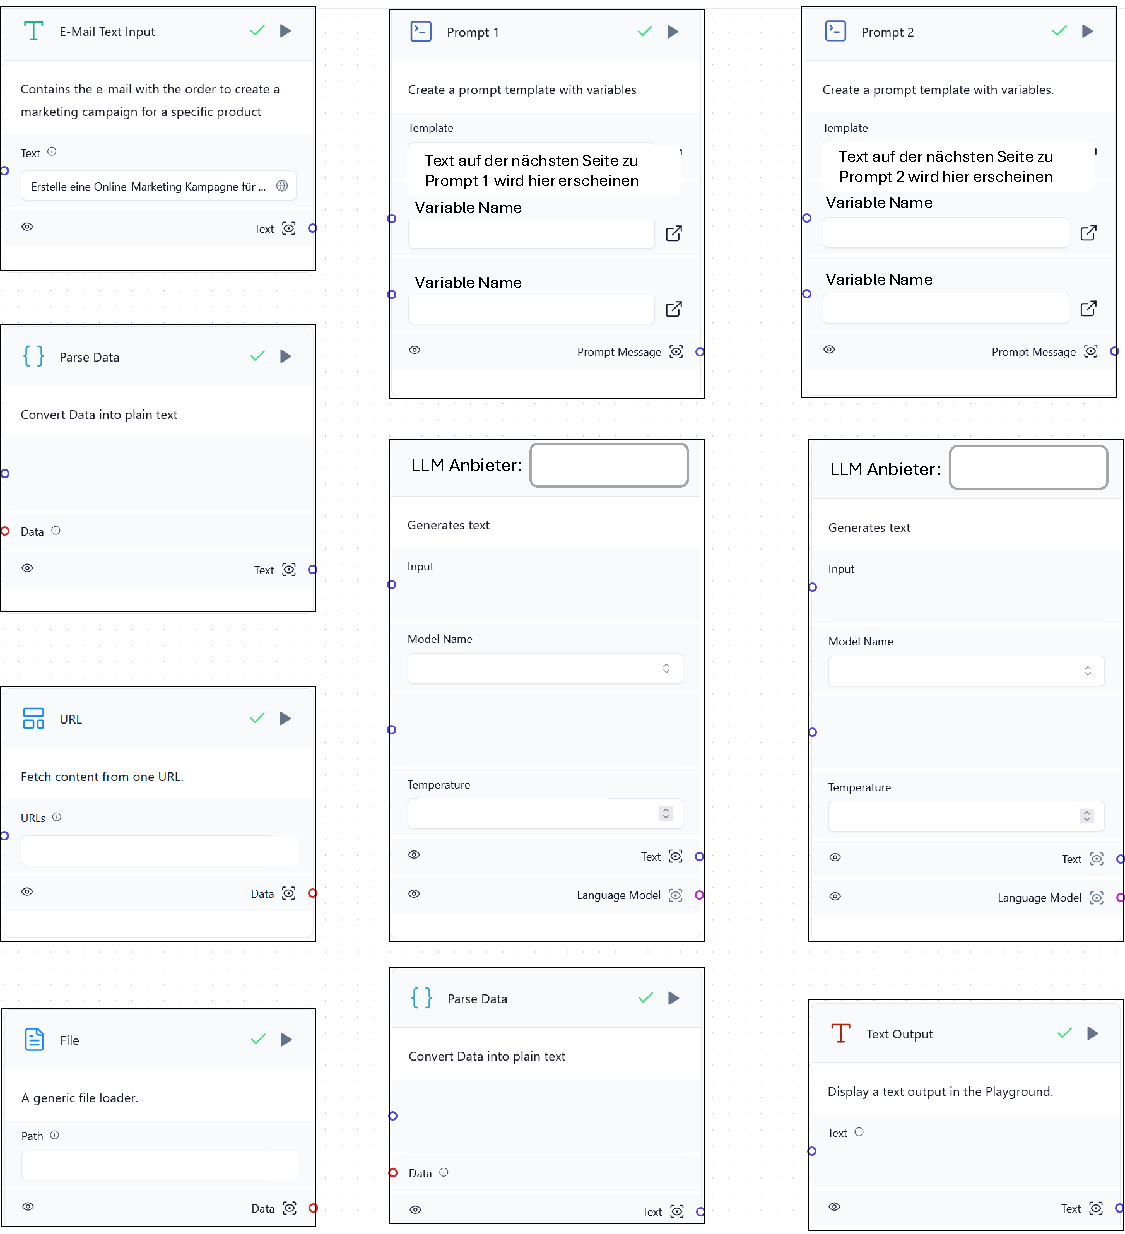
\includegraphics[width=\linewidth]{media/Aufgabe 6/Aufgabe6.pdf}
        \label{fig:Aufgabe6}
        % \caption{Langflow-Komponenten}
    \end{figure}
    %}

    % Aufgabenteil a
    \begin{enumerate}[a)]
		\item 
			\begin{minipage}[t]{\linewidth}
				\vspace{-0.61em}
				\begin{wrapfigure}[2]{r}{0.18\linewidth} 
					\raggedleft
					\texttt{(5 Punkte)}
				\end{wrapfigure}
                Verbinden Sie die auf Seite 9 dargestellten Komponenten sinnvoll miteinander. Füllen Sie fehlende Parameter entsprechend aus.
			\end{minipage}
	\end{enumerate}

	\begin{solution}
		\noindent
                \begin{figure}
                    \centering
                    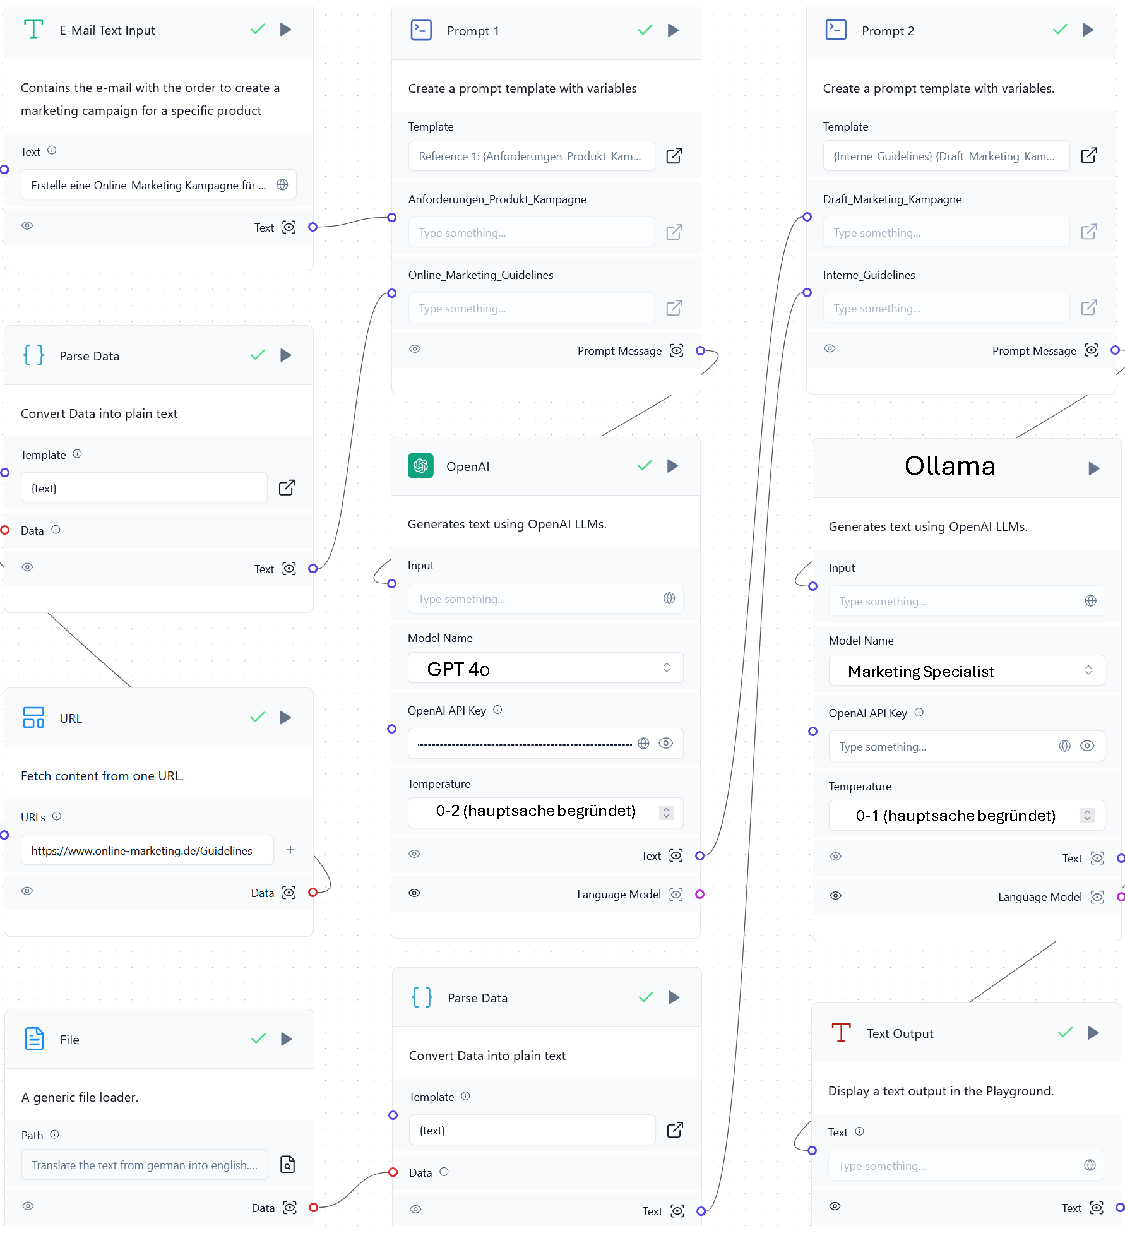
\includegraphics[width=\linewidth]{media/Aufgabe 6/Aufgabe6-Loesung.pdf}
                    % \caption{Sinnvolle Verbindung der Langflow Komponenten}
                    \label{fig:Aufgabe6-Loesung}
                \end{figure}
	\end{solution}


    % Aufgabenteil b
    \begin{enumerate}[b)]
		\item 
			\begin{minipage}[t]{\linewidth}
				\vspace{-0.61em}
				\begin{wrapfigure}[2]{r}{0.18\linewidth} 
					\raggedleft
					\texttt{(1 Punkt)}
				\end{wrapfigure}
                Schreiben Sie den ersten Prompt. Dieser Text wird als Text für die Langflow Komponente Prompt 1 verwendet. Input-Variablen müssen initialisiert und mit geschwungen Klammern verwendet werden, z.B. \{variable\_name\}:
			\end{minipage}
	\end{enumerate}

	\begin{solution}
		\noindent
		\fbox{\parbox[c]{\textwidth}{
				\small
				\begin{tabular}{cp{13cm}}
					Punkte &\\
					1 & Analysiere die Kundenanforderungen für die Produkt-Marketingkampagne: \{Anforderungen\_Produkt\_Kampagne\}
				\end{tabular}
				\hspace{\textwidth}
		}}\\
	\end{solution}

    \begin{answerbox}
		\noindent
		\fbox{\parbox[c]{\textwidth}{
				\vspace{5cm}
				\hspace{\textwidth}
		}}\\
	\end{answerbox}

    % Aufgabenteil c
    \begin{enumerate}[c)]
		\item 
			\begin{minipage}[t]{\linewidth}
				\vspace{-0.61em}
				\begin{wrapfigure}[2]{r}{0.18\linewidth} 
					\raggedleft
					\texttt{(1 Punkt)}
				\end{wrapfigure}
                Schreiben Sie den zweiten Prompt. Dieser Text wird als Text für die Langflow Komponente Prompt 2 verwendet. Input-Variablen müssen initialisiert und mit geschwungen Klammern verwendet werden, z.B. \{variable\_name\}:
			\end{minipage}
	\end{enumerate}

	\begin{solution}
		\noindent
		\fbox{\parbox[c]{\textwidth}{
				\small
				\begin{tabular}{cp{13cm}}
					Punkte &\\
					1 & Überarbeite diesen Entwurf einer Marketingkampagne: \{Draft\_Marketing\_Kampagne\}. Nutze für die Überarbeitungen die internen Informationen aus: \{Interne\_Guidelines\}.
				\end{tabular}
				\hspace{\textwidth}
		}}\\
	\end{solution}

    \begin{answerbox}
		\noindent
		\fbox{\parbox[c]{\textwidth}{
				\vspace{5cm}
				\hspace{\textwidth}
		}}\\
	\end{answerbox}

    % Aufgabenteil d
    \begin{enumerate}[d)]
		\item 
			\begin{minipage}[t]{\linewidth}
				\vspace{-0.61em}
				\begin{wrapfigure}[2]{r}{0.18\linewidth} 
					\raggedleft
					\texttt{(1,5 Punkte)}
				\end{wrapfigure}
                Begründen Sie die Auswahl des ersten LLM-Anbieters, des LLM-Modells und des Temperature Settings:
			\end{minipage}
	\end{enumerate}

	\begin{solution}
		\noindent
		\fbox{\parbox[c]{\textwidth}{
				\small
				\begin{tabular}{cp{13cm}}
					Punkte &\\
					2 & OpenAI mit ChatGPT 4o wurde ausgewählt, weil alle Informationen online verfügbar sind und verfügbar gemacht werden sollen (Guidelines und die Marketing Kampagne). ChatGPt 4o is als Marktführer geeignet, diese Komplexe Aufgabe durchzuführen. Als Temperatur wurde 0 gewählt, damit sich die KI an die Guidelines hält ohne dabei zu wenig oder zu sehr kreativ zu werden.
				\end{tabular}
				\hspace{\textwidth}
		}}\\
	\end{solution}

    \begin{answerbox}
		\noindent
		\fbox{\parbox[c]{\textwidth}{
				\vspace{5cm}
				\hspace{\textwidth}
		}}\\
	\end{answerbox}

     % Aufgabenteil e
    \begin{enumerate}[e)]
		\item 
			\begin{minipage}[t]{\linewidth}
				\vspace{-0.61em}
				\begin{wrapfigure}[2]{r}{0.18\linewidth} 
					\raggedleft
					\texttt{(1,5 Punkte)}
				\end{wrapfigure}
                Begründen Sie die Auswahl des zweiten LLM-Anbieters, des LLM-Modells und des Temperature Settings:
			\end{minipage}
	\end{enumerate}

	\begin{solution}
		\noindent
		\fbox{\parbox[c]{\textwidth}{
				\small
				\begin{tabular}{cp{13cm}}
					Punkte &\\
					2 & Ollama mit Marketing Specialist wurde entsprechend den Anforderungen aus der Aufgabenbeschreibung gewählt. Die Temperatur 0 wurde wieder gewählt, damit sich das eigene LLM an die internen Richtlinien hält, ohne dabei zu wenig oder zu sehr kreativ zu werden.
				\end{tabular}
				\hspace{\textwidth}
		}}\\
	\end{solution}

    \begin{answerbox}
		\noindent
		\fbox{\parbox[c]{\textwidth}{
				\vspace{5cm}
				\hspace{\textwidth}
		}}\\
	\end{answerbox}

\end{document}
